\documentclass[12pt, twoside]{article}
\usepackage[francais]{babel}
\usepackage[T1]{fontenc}
\usepackage[latin1]{inputenc}
\usepackage[left=7mm, right=7mm, top=7mm, bottom=7mm]{geometry}
\usepackage{float}
\usepackage{graphicx}
\usepackage{array}
\usepackage{multirow}
\usepackage{amsmath,amssymb,mathrsfs} 
\usepackage{soul}
\usepackage{textcomp}
\usepackage{eurosym}
\usepackage{lscape}
 \usepackage{variations}
\usepackage{tabvar}
 
\pagestyle{empty}

\title{\ul{\textbf{Angles}}}
\date{}

\begin{document}
\maketitle


\section{Notation des angles}


On note un angle avec trois lettres. La lettre centrale d�signe le
\textbf{sommet} de l'angle.


\bigskip

\ul{Exemples}:

\begin{tabular}{cc}

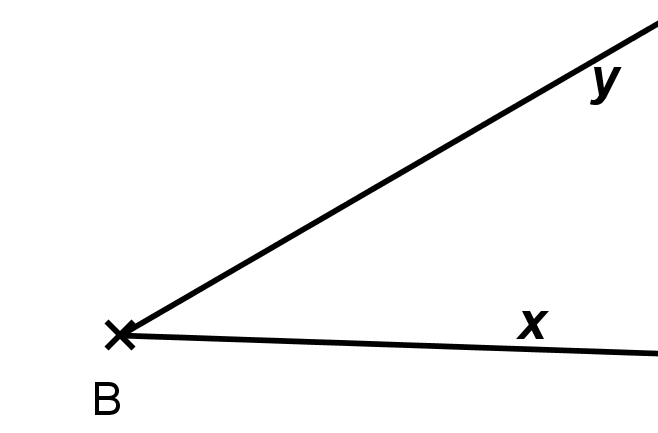
\includegraphics[width=4cm]{images/angle1.png} \qquad \qquad & \qquad \qquad 
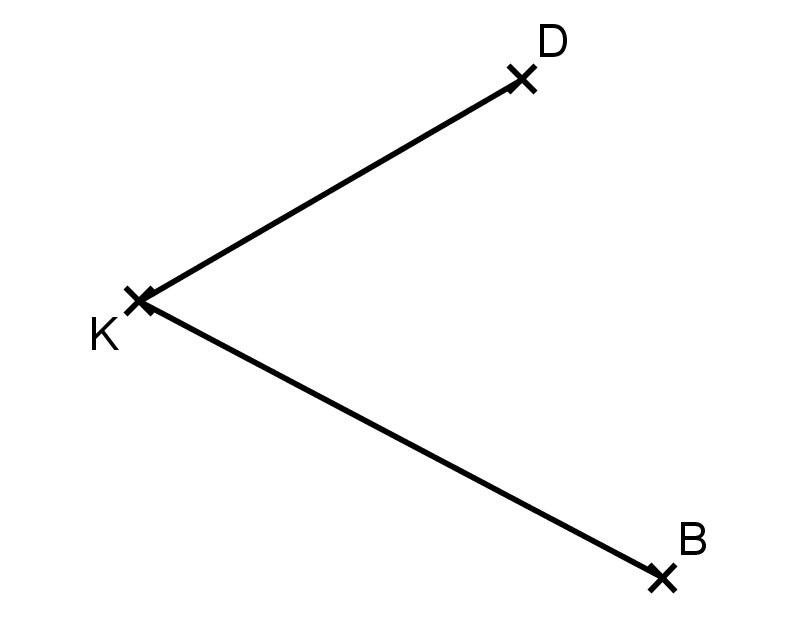
\includegraphics[width=45mm]{images/angle2.png} \\

Cet angle se note $\widehat{xBy}$ ou $\widehat{yBx}$. \qquad \qquad  & \qquad
\qquad  \qquad Cet angle se note $\widehat{DKB}$ ou $\widehat{BKD}$. \\
\end{tabular}




\section{Codage des angles de m�me mesure}


Le codage indique que les angles $\widehat{AED}$ et $\widehat{FDE}$ ont la m�me
mesure.

On note: $\widehat{AED}=\widehat{FDE}$.


\section{Mesure d'un angle}

\subsection{Le degr�}


Pour mesurer des angles, on utilise un \textbf{rapporteur}. Le rapporteur est
gradu� en \textbf{degr�s}.


15 degr�s se note 15�. 


\bigskip

\ul{M�thode pour mesurer un angle � l'aide du rapporteur:}

\enskip

\begin{center}
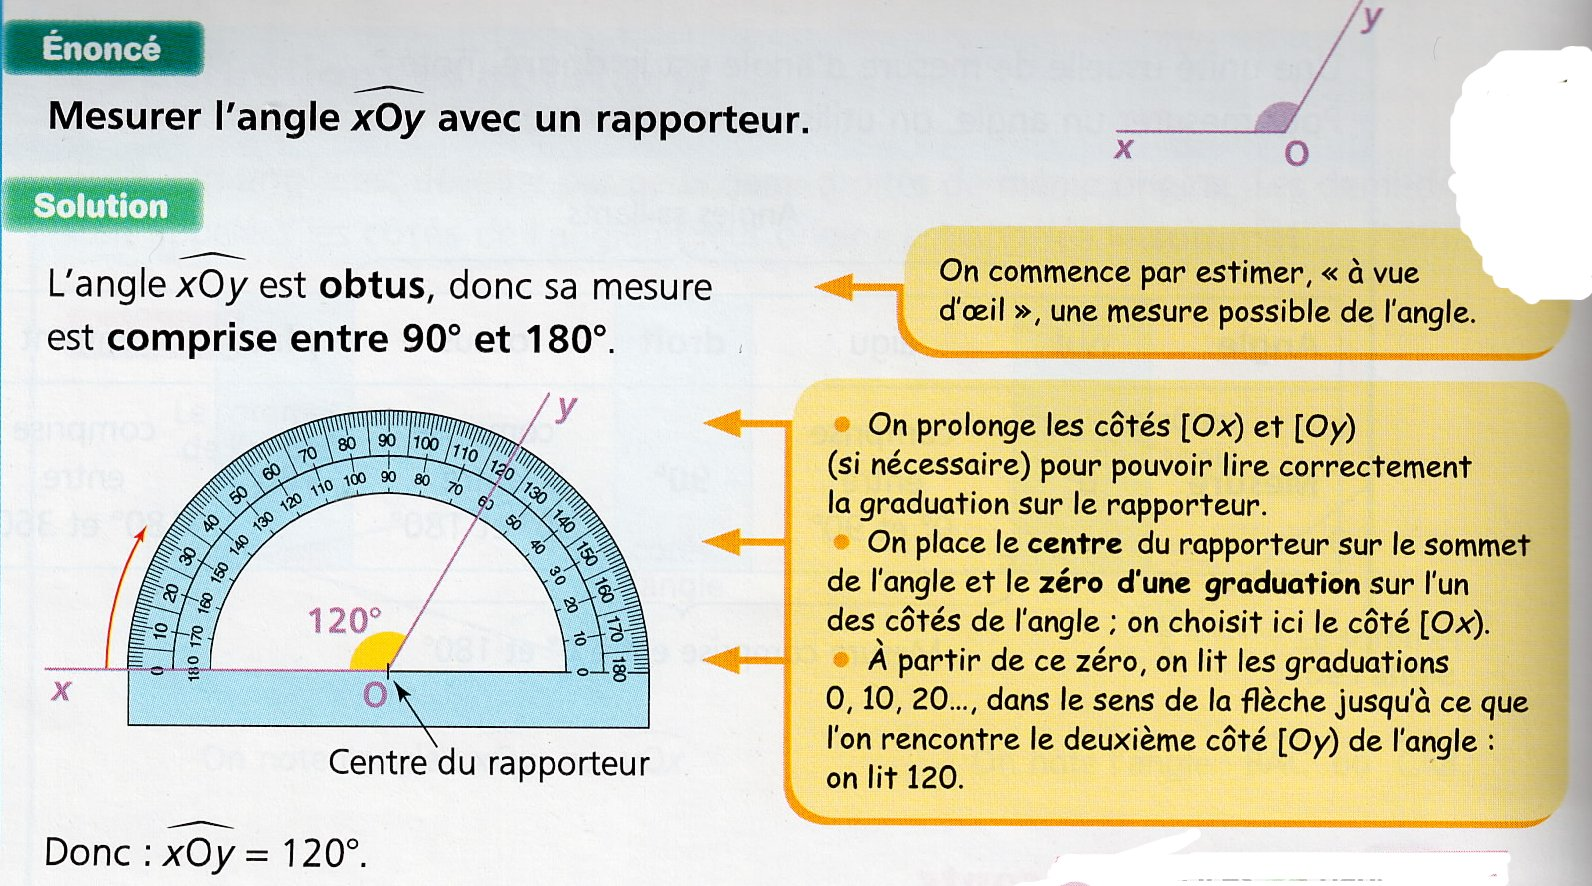
\includegraphics[width=12cm]{images/methode_rapporteur.jpg}
\end{center}


\subsection{Angles particuliers}

\begin{center}
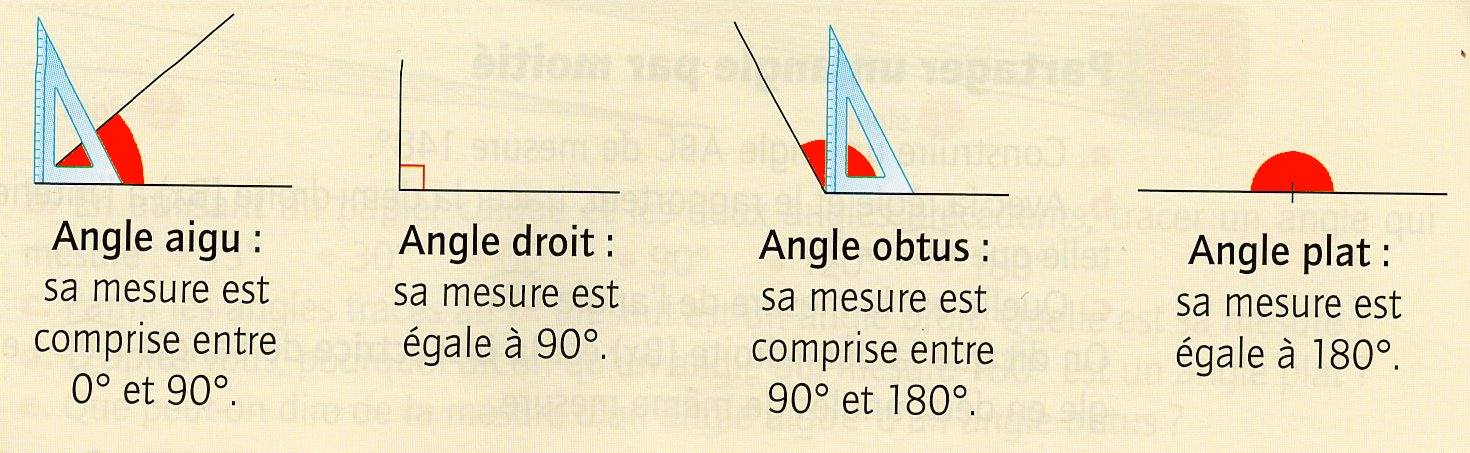
\includegraphics[width=12cm]{images/angles_particuliers.jpg}
\end{center}


\subsection{M�thode pour construire un angle de mesure donn�e}

\ul{Exemple}: Tracer un angle $\widehat{xBy}$ de mesure 45�.


\enskip

\ul{M�thode}:


\begin{enumerate}
  \item On trace l'un des c�t�s de l'angle par exemple la demi-droite [Bx).
  \item On place le centre du rapporteur sur l'origine B et la graduation ``0''
  sur le c�t� [Bx). On suit cette graduation (0; 10; 20 \ldots) et on fait une
  marque � la graduation 45.
  \item On trace la demi-droite [By) qui passe par la marque faire pr�cedemment.
\end{enumerate}  





\bigskip

\bigskip

\bigskip

\bigskip

\bigskip

\bigskip

\bigskip

\bigskip

\bigskip


\section{Bissectrice d'un angle}



\ul{D�finition}: La \textbf{bissectrice} d'un angle est la demi-droite qui
partage cet angle en \textbf{deux angles de m�me mesure}.


\bigskip

\ul{M�thode 1}: avec le rapporteur et la r�gle

\enskip

\begin{center}
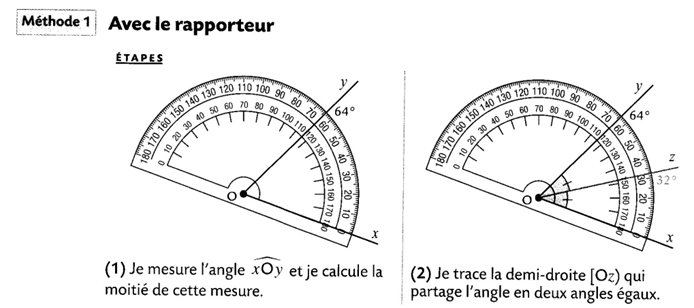
\includegraphics[width=14cm]{images/methode1.jpg}
\end{center}

\bigskip



\ul{Exemple}: Trace la bissectrice de l'angle $\widehat{xOy}$ � l'aide du
rapporteur.




\begin{center}
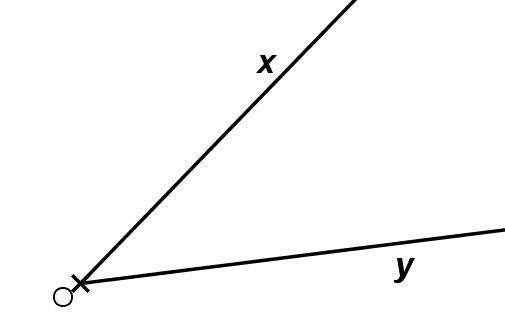
\includegraphics[width=5cm]{images/bissec1.png}
\end{center}

\bigskip


\bigskip


\ul{M�thode 2}: avec le compas et la r�gle

\enskip 

\begin{center}
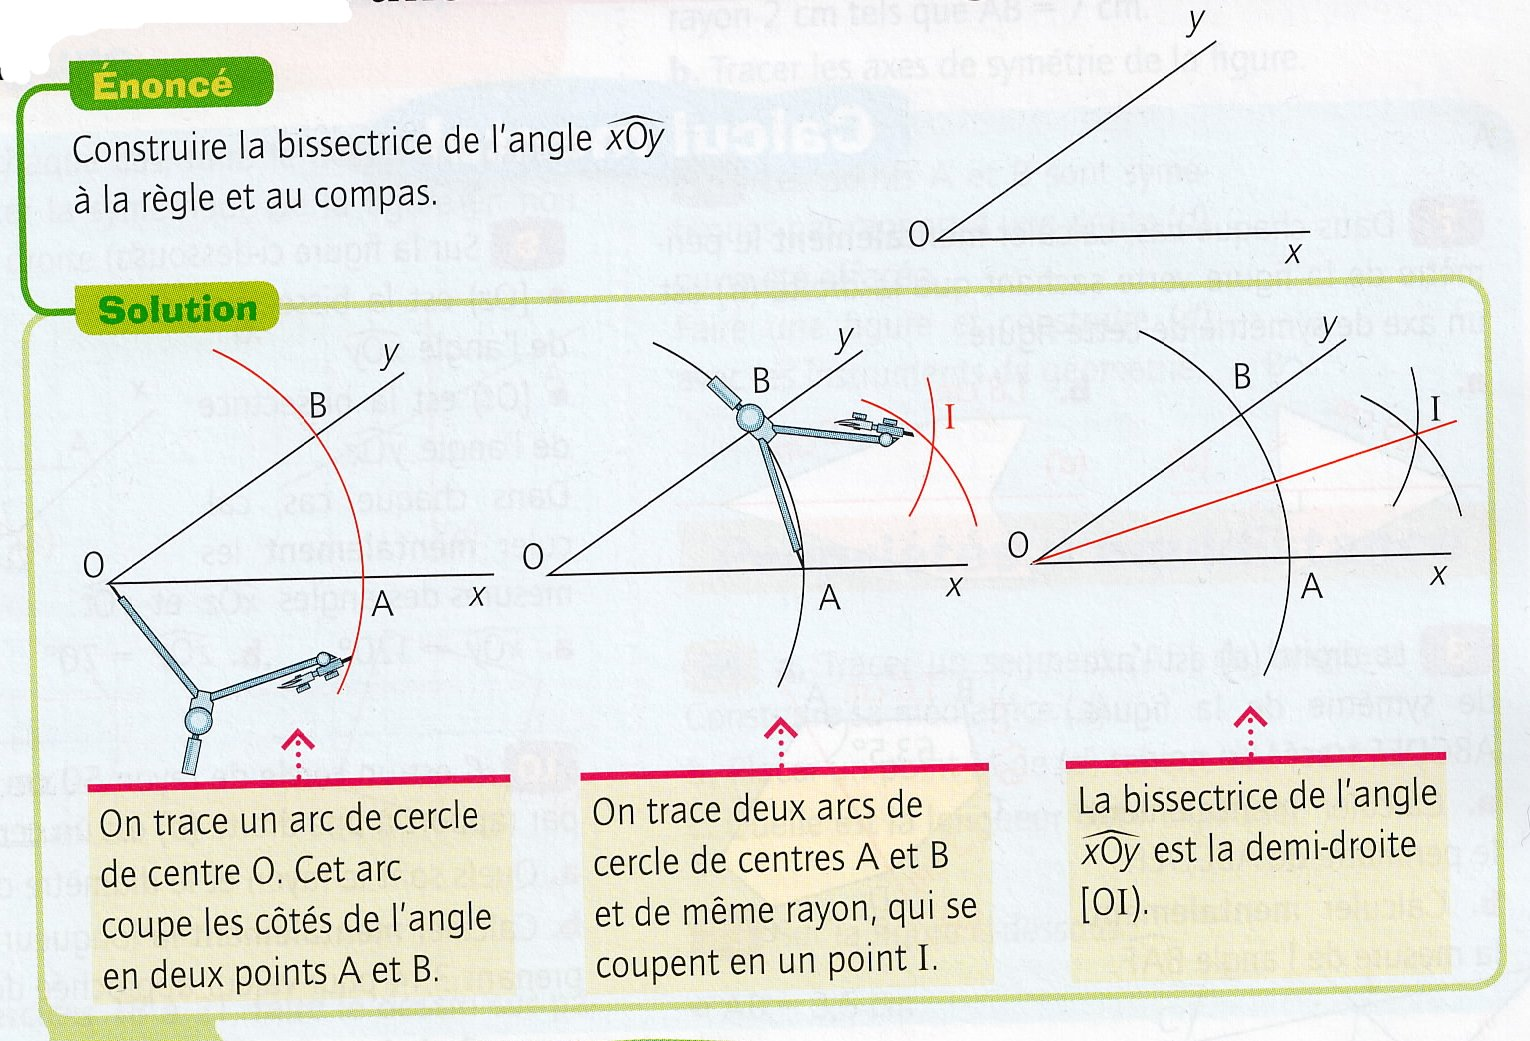
\includegraphics[width=12cm]{images/methode2.jpg}
\end{center} 


\bigskip

\ul{Exemple}: Trace la bissectrice de l'angle $\widehat{xOy}$ � l'aide du
compas.

 
\begin{center}
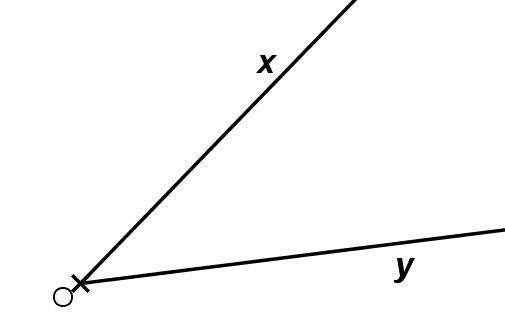
\includegraphics[width=5cm]{images/bissec1.png}
\end{center}
\end{document}
